\begin{figure}[h]
    \centering
    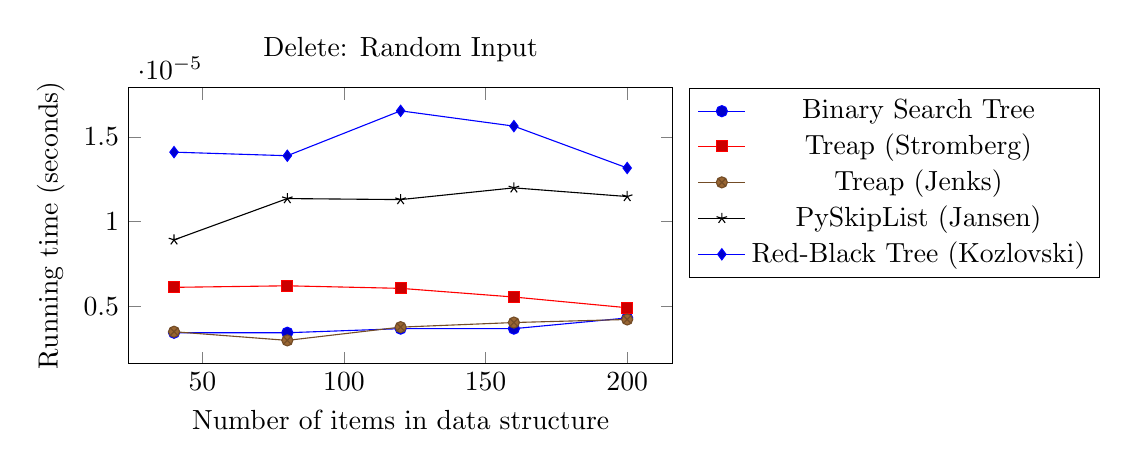
\begin{tikzpicture}
        \begin{axis}[
            xlabel={Number of items in data structure},
            ylabel={Running time (seconds)},
            title={Delete: Random Input},
            width=0.7\textwidth,
            height=2in,
            legend pos=outer north east
        ]
		\addplot coordinates {
			(200, 4.306807315548932e-06)
			(160, 3.6743391083704157e-06)
			(120, 3.6743391083704157e-06)
			(80, 3.4333988389690513e-06)
			(40, 3.4333988389690513e-06)
		};
		\addplot coordinates {
			(200, 4.909157989052212e-06)
			(160, 5.541626196230859e-06)
			(120, 6.053624268708649e-06)
			(80, 6.204211937084481e-06)
			(40, 6.113859336059034e-06)
		};
		\addplot coordinates {
			(200, 4.216454714523442e-06)
			(160, 4.035749512472375e-06)
			(120, 3.764691709395862e-06)
			(80, 2.9816358338414716e-06)
			(40, 3.4936339063195223e-06)
		};
		\addplot coordinates {
			(200, 1.1474780330238826e-05)
			(160, 1.1986778402716531e-05)
			(120, 1.129407512818776e-05)
			(80, 1.1354310195538057e-05)
			(40, 8.914789967849439e-06)
		};
		\addplot coordinates {
			(200, 1.3161362216048203e-05)
			(160, 1.5630999977411796e-05)
			(120, 1.6534525987666956e-05)
			(80, 1.3884183024252122e-05)
			(40, 1.4095005759978338e-05)
		};
        \legend{Binary Search Tree, Treap (Stromberg), Treap (Jenks), PySkipList (Jansen), Red-Black Tree (Kozlovski)}
        \end{axis}
    \end{tikzpicture}
    \caption{Average of 10 operations, benchmarked every 40, starting at 40.}
\end{figure}